\renewcommand{\thechapter}{1}
\chapter{Theory of \texorpdfstring{$\beta\beta 0\nu$}{Neutrinoless Double-Beta} Decay}

\tikzstyle{ParticleInteraction}=[coordinate]
\tikzstyle{ParticleLabel}=[]

\begin{figure}
\begin{center}
\begin{tikzpicture}

\node[ParticleLabel] (u1) {u};
\node[ParticleLabel] (e1) [below of=u1] {$e^{-}$};
\node[ParticleLabel] (nu1) [below of=e1] {$\overline{\nu}$};
\node[ParticleInteraction] (Weak1) [left of=e1] {};
\node[ParticleInteraction] (Strong1) [above left of=Weak1] {};
\node[ParticleLabel] (d1) [left of=Strong1] {d};

\node[ParticleLabel] (nu2) [below of=nu1] {$\overline{\nu}$};
\node[ParticleLabel] (e2) [below of=nu2] {$e^{-}$};
\node[ParticleLabel] (u2) [below of=e2] {u};
\node[ParticleInteraction] (Weak2) [left of=e2] {};
\node[ParticleInteraction] (Strong2) [below left of=Weak2] {};
\node[ParticleLabel] (d2) [left of=Strong2] {d};

\draw (Weak1) -- (nu1) node[midway,sloped] {$<$};
\draw (Strong1) -- (u1) node[midway,sloped] {$>$};
\draw[snake=snake] (Strong1) -- (Weak1) node[midway,below left] {$W^{-}$};
\draw (Weak1) -- (e1) node[midway,sloped] {$>$};
\draw (d1) -- (Strong1) node[midway,sloped] {$>$};

\draw (Weak2) -- (nu2) node[midway,sloped] {$<$};
\draw (Strong2) -- (u2) node[midway,sloped] {$>$};
\draw[snake=snake] (Strong2) -- (Weak2) node[midway,above left] {$W^{-}$};
\draw (Weak2) -- (e2) node[midway,sloped] {$>$};
\draw (d2) -- (Strong2) node[midway,sloped] {$>$};

\end{tikzpicture}
\end{center}
\caption{Feynman diagram for $\beta\beta 2 \nu$ decay.  The reaction products are equivalent to two $\beta$ decays in succession, but this reaction can occur even if a single $\beta$ decay would be energetically forbidden.}
\label{fig:FeynmanBetaBeta2Nu}
\end{figure}

\begin{figure}
\begin{center}
\begin{tikzpicture}

\node[ParticleLabel] (u1) {u};
\node[ParticleLabel] (e1) [below of=u1] {$e^{-}$};
\node[ParticleInteraction] (Weak1) [left of=e1] {};
\node[ParticleInteraction] (Strong1) [above left of=Weak1] {};
\node[ParticleLabel] (d1) [left of=Strong1] {d};

\node[ParticleLabel] (nu) [below of=Weak1] {$\times$};

\node[ParticleInteraction] (Weak2) [below of=nu] {};
\node[ParticleLabel] (e2) [right of=Weak2] {$e^{-}$};
\node[ParticleLabel] (u2) [below of=e2] {u};
\node[ParticleInteraction] (Strong2) [below left of=Weak2] {};
\node[ParticleLabel] (d2) [left of=Strong2] {d};

\draw (Strong1) -- (u1) node[midway,sloped] {$>$};
\draw[snake=snake] (Strong1) -- (Weak1) node[midway,below left] {$W^{-}$};
\draw (Weak1) -- (e1) node[midway,sloped] {$>$};
\draw (d1) -- (Strong1) node[midway,sloped] {$>$};

\draw[dashed] (Weak1) -- (nu) node[at end,right] {$\nu_M$};
\draw[dashed] (Weak2) -- (nu);

\draw (Strong2) -- (u2) node[midway,sloped] {$>$};
\draw[snake=snake] (Strong2) -- (Weak2) node[midway,above left] {$W^{-}$};
\draw (Weak2) -- (e2) node[midway,sloped] {$>$};
\draw (d2) -- (Strong2) node[midway,sloped] {$>$};

\end{tikzpicture}
\end{center}
\caption{Feynman diagram for $\beta\beta 0 \nu$ decay.  A virtual neutrino mediates the exchange.  This is only possible if $\overline{\nu}_R$ can oscillate to $\nu_L$, and the interaction that induces this oscillation also generates neutrino mass.}
\label{fig:FeynmanBetaBeta0Nu}
\end{figure}

\begin{table}
\begin{center}
\begin{tabular}{|rccc|}
\hline Isotope & \shortstack{$\beta\beta 0\nu$ Halflife Limit \\ ($90\%$ CL, in years)} & Collaboration & Citation \\ \hline
$^{48}$Ca & $1.3 \cdot 10^{22}$ & NEMO-3 & \cite{NEMO2011RandomOtherIsotopes}\\
$^{76}$Ge & $2.1 \cdot 10^{25}$ & GERDA & \cite{PhysRevLett.111.122503} \\
$^{82}$Se & $3.6 \cdot 10^{23}$ & NEMO-3 & \cite{NEMO2011RandomOtherIsotopes}\\
$^{96}$Zr & $9.2 \cdot 10^{21}$ & NEMO-3 & \cite{Argyriades2010168}\\
$^{100}$Mo & $1.1 \cdot 10^{24}$ & NEMO-3 & \cite{NEMO3-2013-100Mo}\\
$^{116}$Cd & $1.6 \cdot 10^{22}$ & NEMO-3 & \cite{NEMO2011RandomOtherIsotopes}\\
$^{130}$Te & $3.0 \cdot 10^{24}$ & Cuoricino & \cite{PhysRevC.78.035502}\\
$^{136}$Xe & \textcolor{red}{FILL IN} & & \\
$^{136}$Xe & $1.9 \cdot 10^{25}$ & KamLAND-Zen & \cite{PhysRevLett.110.062502}\\
$^{150}$Nd & $1.8 \cdot 10^{22}$ & NEMO-3 & \cite{PhysRevC.80.032501}\\
\hline
\end{tabular}
\end{center}
\caption{A listing of the strongest available $\beta\beta 0\nu$ limits.  $\beta\beta$ isotopes with no known limits on $\beta\beta 0\nu$ are not listed.  For $^{136}$Xe, this author has taken the liberty of including the most recent results from both EXO-200 and Kamland-Zen.}
\label{tab:0nubb_limits}
\end{table}

Standard-model $\beta\beta$ decay is the result of the particle interaction $2d \rightarrow 2u + 2e^- + 2\bar{\nu}_e$ mediated by $W^-$-exchange, as depicted in Figure~\ref{fig:FeynmanBetaBeta2Nu}.  It is effectively the simultaneous occurance of two $\beta$ decays from the same nucleus.

$\beta\beta$ decay is the result of a second-order weak interaction, so it has a remarkably long half-life; however, it does not violate any fundamental symmetries and is, in this sense, a mundane prediction of the Standard Model.  Although many nuclei are expected to decay by $\beta\beta$, the process is thoroughly masked by conventional $\beta$ decay in most of them.  We can only hope to detect $\beta\beta$ decay in isotopes where single-$\beta$ decay is forbidden or highly suppressed.

In rare cases, single-$\beta$ decay may be highly suppressed, enabling $\beta\beta$ decay to have a rate comparable to or exceeding single-$\beta$ decay.  This is, for example, the case in $^{48}_{20}$Ca: the ground state of $^{48}_{20}$Ca has zero units of angular momentum, whereas its single-$\beta$-decay daughter product $^{48}_{21}$Sc has six units of total angular momentum in its ground state.  This $\beta$ decay is thus highly suppressed by angular momentum conservation.  By contrast, $^{48}_{22}$Ti has zero units of total angular momentum, making $\beta\beta$ decay of $^{48}_{20}$Ca permitted by angular momentum considerations, and as a result the $\beta\beta$ decay mode of $^{48}_{20}$Ca is expected to be dominant.~\cite{MyNuclearPhysicsBook}

However, generally the suppression of single-$\beta$ decay comes in the form of energy conservation.  It is well-known that nuclei minimize their energy by arranging similar nucleons to have overlapping wavefunctions.~\cite{MyNuclearPhysicsBook}  Thus, isotopes with an even number of protons and an even number of neutrons will have less nucleon-pairing potential energy than an isotope with either an odd number of protons or an odd number of neutrons, which in turn will have less nucleon-pairing potential energy than an isotope with an odd number of protons and an odd number of electrons.

\begin{figure}
\begin{center}
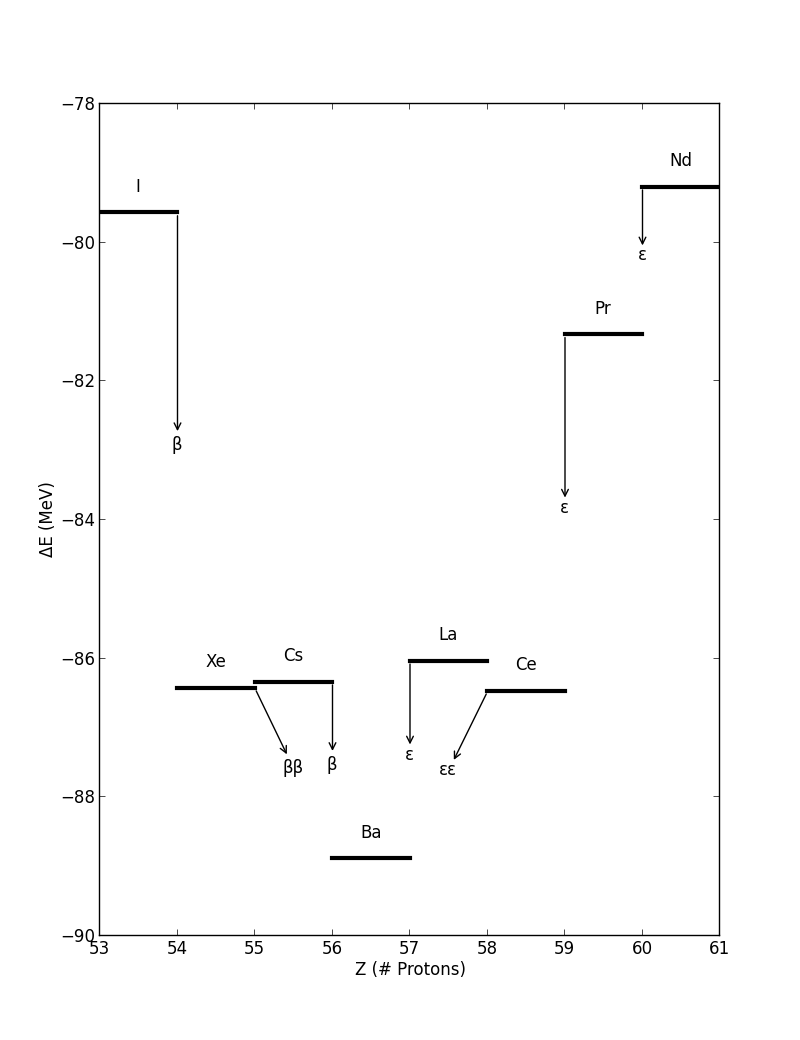
\includegraphics[keepaspectratio=true,width=\textwidth]{scripts/LevelDiagram.png}
\end{center}
\renewcommand{\baselinestretch}{1}
\small\normalsize
\begin{quote}
\caption{Energy diagram of isotopes with atomic mass $A=136$.  Values are from~\cite{AtomicMassEvaluation}.  The energies $\Delta E$ are the binding energies of the atom, compared to the bare masses of the same nuclei.}
\label{fig:LevelDiagram}
\end{quote}
\end{figure}
\renewcommand{\baselinestretch}{2}
\small\normalsize

A typical nuclear energy level diagram is shown in figure~\ref{fig:LevelDiagram} for the $A=136$ isobar: Xenon, Barium, Cerium, and Neodynium are even-even isotopes, and have systematically lower energies than the odd-odd isotopes Iodine, Cesium, Lanthanum, and Praseodymium.  For this particular isobar, we can see that Xenon is energetically forbidden from single-$\beta$ decaying to Cesium because the odd-odd isotope of Cesium has just slightly more potential energy than the even-even isotope of Xenon; as a result, the primary mode of decay of Xenon-136 will be by $\beta\beta$ decay to Barium-136.  (We also note a similar feature, that the primary mode of decay of Cerium-136 will be by double-electron-capture ($\epsilon\epsilon$) to Barium-136.  Many of the same implications of $\beta\beta$ decay also apply to $\epsilon\epsilon$ decay; however, in practice the rates for these decays will be lower than the rates for $\beta\beta$ decay, so we will not consider them further in this work.)

The detection and study of $\beta\beta$ decay provides an opportunity to test a new class of nuclear matrix computations; however, the primary appeal of $\beta\beta$ decay is through the opportunity it provides to probe the nature of neutrinos.  It has been suggested as early as 1937 that neutrinos could possess mass through a neutrino-antineutrino interaction, provided that the neutrino be its own antiparticle~\cite{Majorana}.  As evidence mounted through the 1990's that neutrinos must have nonzero mass (see, in particular, the observation of neutrino oscillation in ~\cite{SuperK}), interest in possible mass-generating mechanisms has increased -- including Majorana's mechanism.

If neutrinos do have Majorana mass interactions, then any isotope that undergoes $\beta\beta$ decay can also undergo the related process $2d \rightarrow 2u + 2e^-$, depicted in Figure~\ref{fig:FeynmanBetaBeta0Nu}, in which the two outgoing neutrinos in $\beta\beta$ decay are replaced by one virtual neutrino.  We can interpret this as a mixing interaction between a left-handed neutrino and a right-handed antineutrino; this is only possible if neutrinos are Majorana particles.  We refer to the standard process as $\beta\beta 2\nu$ decay and the novel process as $\beta\beta 0\nu$ decay.

A clear observation of $\beta\beta 0\nu$ decay would immediately yield a number of interesting physical insights.  The existence of the process automatically demonstrates non-conservation of total lepton number, since the lepton number changes by 2 in a Majorana interaction.  Numerous theories have suggested other plausible modes of lepton number non-conservation~\cite{ProtonDecay}\cite{MuonToPositron}, but none have yet reported a positive result.  In the conventional Standard Model with massless neutrinos, lepton number conservation is an accidental symmetry~\cite{LeptonConservation}, but since neutrinos are known to have mass, there is no longer \textit{a priori} any reason to expect conservation or non-conservation.

A second conclusion, as discussed above, would be that neutrino mass comes from a Majorana mass term.  This term appears in the Lagrangian (for each mass eigenstate) as 
\begin{align}
\mathcal{L}_{Maj}&= \begin{aligned}[t]
 & -\frac{m_{L}}{2} \left( \overline{\Psi_L^c} \Psi_L^{} + \overline{\Psi_L^{}} \Psi_L^c \right)\\
 & -\frac{m_{R}}{2} \left( \overline{\Psi_R^c} \Psi_R^{} + \overline{\Psi_R^{}} \Psi_R^c \right),
\end{aligned}
\end{align}
where the superscript-$c$ represents charge conjugation.  (This is the reason that Majorana mass terms are only possible for a chargeless lepton.)  The masses $m_L$ and $m_R$ may be tuned independently; since there has never been an observation of right-handed neutrinos or left-handed anti-neutrinos, it is possible that $m_R = 0$ and that the fields $\Psi_R^{}$ and $\Psi_R^c$ do not exist in nature~\cite{RMPbb0n}.

\begin{figure}
\begin{center}
\begin{tikzpicture}

\node[circle,fill=black,pattern=dots,minimum size=100] (BlackBox) {};
\node (e1) at ([shift={(30:3)}]BlackBox) {$e^{-}$};
\node (e2) at ([shift={(-30:3)}]BlackBox) {$e^{-}$};
\node (u1) at ([shift={(60:3)}]BlackBox) {u};
\node (u2) at ([shift={(-60:3)}]BlackBox) {u};
\node (d1) at ([shift={(120:3)}]BlackBox) {d};
\node (d2) at ([shift={(-120:3)}]BlackBox) {d};

\draw (d1) -- (BlackBox) node[midway,sloped] {$>$};
\draw (d2) -- (BlackBox) node[midway,sloped] {$>$};
\draw (BlackBox) -- (u1) node[midway,sloped] {$>$};
\draw (BlackBox) -- (u2) node[midway,sloped] {$>$};
\draw (BlackBox) -- (e1) node[midway,sloped] {$>$};
\draw (BlackBox) -- (e2) node[midway,sloped] {$>$};
\end{tikzpicture}
\end{center}
\caption{A generic $\beta\beta 0\nu$ process, with no assumptions of the underlying mechanism.  If $\beta\beta 0\nu$ is observed, it requires that this reaction is possible even though it does not strictly imply that the oscillation in Figure~\ref{fig:FeynmanBetaBeta0Nu} is the cause.}
\label{fig:FeynmanBetaBeta0NuBlob}
\end{figure}

\begin{figure}
\begin{center}
\begin{tikzpicture}
\node[circle,fill=black,pattern=dots,minimum size=30] (BlackBox) {};
\node[coordinate] (Strong1) at ([shift={(180:2)}]BlackBox) {};
\node[coordinate] (Strong2) at ([shift={(0:2)}]BlackBox) {};
\node[coordinate] (Weak1) [left of=Strong1] {};
\node[coordinate] (Weak2) [right of=Strong2] {};
\node (Nu1) [left of=Weak1] {$\overline{\nu}$};
\node (Nu2) [right of=Weak2] {$\nu$};

\draw[-,out=120,in=90] (BlackBox) to node[midway,sloped]{$<$} node[above]{$\overline{u}$} (Strong1) ;
\draw[-,out=-90,in=-120] (Strong1) to node[midway,sloped]{$>$} node[above]{d} (BlackBox);
\draw[-,out=60,in=90] (BlackBox) to node[midway,sloped]{$<$} node[above]{$\overline{d}$} (Strong2) ;
\draw[-,out=-90,in=-60] (Strong2) to node[midway,sloped]{$>$} node[above]{u} (BlackBox);
\draw[snake=snake] (Strong1) to node[above]{$W^{-}$} (Weak1);
\draw[snake=snake] (Strong2) to node[above]{$W^{+}$} (Weak2);
\draw[-,out=-100,in=-90] (BlackBox) to node[midway,sloped]{$>$} node[below]{$e^{+}$} (Weak1);
\draw[-,out=-80,in=-90] (BlackBox) to node[midway,sloped]{$>$} node[below]{$e^{-}$} (Weak2);
\draw[-] (Weak1) to node[midway,sloped]{$<$} (Nu1);
\draw[-] (Weak2) to node[midway,sloped]{$>$} (Nu2);

\end{tikzpicture}
\end{center}
\caption{Since $\beta\beta 0\nu$ requires that the reaction in Figure~\ref{fig:FeynmanBetaBeta0NuBlob} occurs, we can insert that diagram into this larger one and assert that regardless of the underlying mechanism, $\beta\beta 0\nu$ implies an effective neutrino mass generated by $\overline{\nu}$-$\nu$ oscillation as a higher-order process.}
\label{fig:FeynmanBetaBeta0NuImplication}
\end{figure}

It is worth noting that the interaction term above assumes no mediating particles in the mechanism, whereas it is possible that $\beta\beta 0\nu$ could be mediated by some higher-order interaction terms.  However, if $\beta\beta 0\nu$ decay is observed, it leads very generally to a conclusion that neutrinos have an \emph{effective} Majorana mass interaction~\cite{BlackBoxTheorem}.  We can see this by examining the generic diagram for $\beta\beta 0\nu$ decay in figure~\ref{fig:FeynmanBetaBeta0NuBlob}.  No matter what the mechanism of the decay is, we can insert this diagram into figure~\ref{fig:FeynmanBetaBeta0NuImplication} and see that an effective neutrino-antineutrino mass vertex is implied by the existence of $\beta\beta 0\nu$ decay.

If the mechanism of $\beta\beta 0\nu$ decay really is, at tree level, a neutrino mass term as shown in Figure~\ref{fig:FeynmanBetaBeta0Nu}, then it is possible to infer the mass scale of the neutrino from the observed rate of decay.  To lowest order we can assert that
\begin{equation} \label{eq:DestructiveMassInteraction}
\left[T^{0\nu}_{1/2}\right]^{-1} \propto \left< m_{\beta\beta} \right>^2 = \left|\Sigma_k m_k U_{ek}^2\right|^2,
\end{equation}
where $U_{ek}$ is the neutrino mixing matrix and the $m_k$ identify the three neutrino mass eigenstates.  The constant of proportionality is isotope-dependent; state-of-the-art nuclear matrix computations can provide it within a factor of $2-3$~\cite{RMPbb0n}.  We will not consider the complex challenges of these computations here.

The neutrino mixing matrix $\mathbf{U}$ is often parametrized as:
\begin{equation}
\mathbf{U} =
\begin{aligned}
\begin{pmatrix}
1 & 0 & 0 \\
0 & cos(\theta_{23}) & sin(\theta_{23}) \\
0 & -sin(\theta_{23}) & cos(\theta_{23})
\end{pmatrix}
\begin{pmatrix}
cos(\theta_{13}) & 0 & sin(\theta_{13})e^{-i\delta} \\
0 & 1 & 0 \\
-sin(\theta_{13})e^{i\delta} & 0 & cos(\theta_{13})
\end{pmatrix} \times \\
\begin{pmatrix}
cos(\theta_{12}) & sin(\theta_{12}) & 0 \\
-sin(\theta_{12}) & cos(\theta_{12}) & 0 \\
0 & 0 & 1
\end{pmatrix}
\begin{pmatrix}
e^{i\alpha_1/2} & 0 & 0 \\
0 & e^{i\alpha_2/2} & 0 \\
0 & 0 & 1
\end{pmatrix}.
\end{aligned}
\end{equation}
Out of the six parameters used in defining this matrix, the only ones which have been measured are $sin^2(2\theta_{12}) = 0.857^{+0.023}_{-0.025}$~\cite{PhysRevD.83.052002}, $sin^2(2\theta_{13}) = 0.089 \pm 0.010 \pm 0.005$~\cite{1674-1137-37-1-011001}, and $sin^2(2\theta_{23}) > 0.95$~\cite{PhysRevLett.107.241801}.

\begin{figure}
\begin{center}
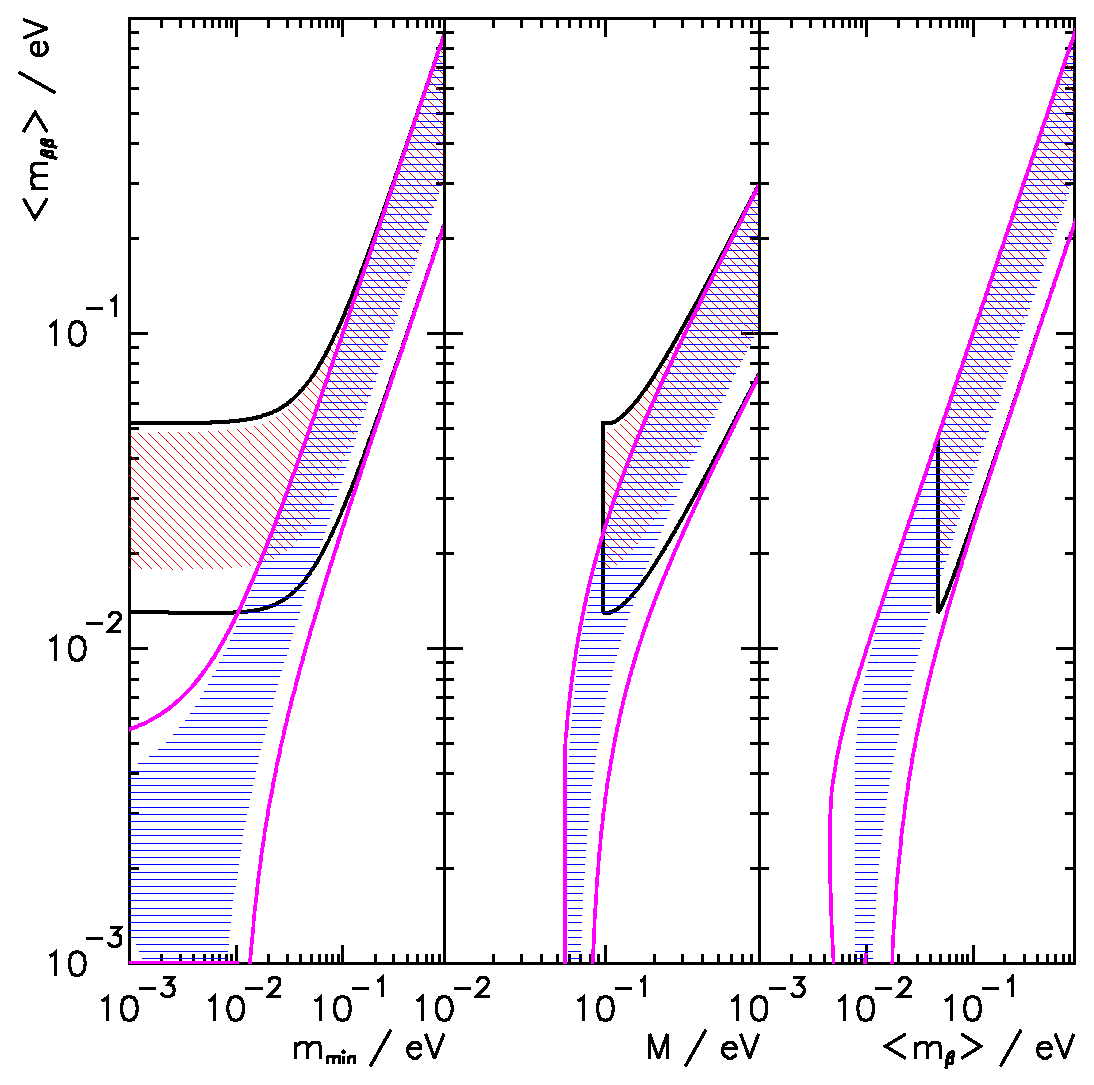
\includegraphics[keepaspectratio=true,width=\textwidth]{PDGNeutrinoMassBounds.eps}
\end{center}
\caption{The relationship between the effective Majorana mass $\left<m_{\beta\beta}\right>$ and other fundamental neutrino quantities: the lightest neutrino mass eigenstate $m_{min}$, the sum of mass eigenstates $M = \sum m_i$, and the effective single-beta-decay neutrino mass $\left<m_{\beta}\right>$.  Black (magenta) lines indicate the allowed region for the inverted (normal) hierarchy; red (blue) hatches indicate uncertainty for the inverted (normal) hierarchy due to the unknown CP-violating and Majorana phases $\delta$, $\alpha_1$, and $\alpha_2$.~\cite{PDG}}
\label{fig:NeutrinoMassBounds}
\end{figure}

For the purpose of $\beta\beta 0\nu$ searches, the most important implication of equation~\ref{eq:DestructiveMassInteraction} is that $\left< m_{\beta\beta}\right>^2$ is a coherent sum of the masses of the neutrino mass eigenstates.  Even though it is known that neutrinos have mass, it is possible for $\left< m_{\beta\beta}\right>^2$ to be arbitrarily small or zero if $\mathbf{U}$ is tuned to create cancellations between the neutrino mass terms.  Figure~\ref{fig:NeutrinoMassBounds} illustrates the relation between $\left< m_{\beta\beta}\right>^2$ and other fundamental neutrino parameters.  We can see that the sum of neutrino masses, $M = \sum m_i$, can be as large as roughly $0.08$ meV without ruling out the possibility of cancellations from $\mathbf{U}$ leading to an extremely small value for $\left< m_{\beta\beta}\right>^2$; conversely, it is possible that neutrinos may be Majorana particles, yet the search to detect $\beta\beta 0\nu$ decay may be hopelessly difficult because of an unfortunate cancellation of terms in the effective Majorana mass.

WORKING FROM HERE.

There are bounds on the values that may be seen, based on previous results in $\beta\beta 0\nu$ decay and other measurements.  Figure~\ref{fig:NeutrinoMassBounds} shows how the various mass parameters can be related to each other.  $M$, the combined masses of all three neutrino flavors, can be limited by cosmological observations; recent results from Planck combined with WMAP and baryon acoustic oscillations have restricted $M < 0.23$ eV ~\cite{CosmologicalLimits}.  Measurements of the $\beta$ decay spectrum of Tritium have yielded bounds on $\left< m_\beta \right>$, the weighted average mass of the electron-neutrino; this parameter is currently known to be less than $2.5$ eV~\cite{OldTritium}, and the KATRIN experiment is expected to begin data-taking in 2012 with a sensitivity down to $0.2$ eV~\cite{NewTritium}.

The strongest limits on $\left< m_{\beta\beta} \right>$ have been published by the Heidelberg-Moscow experiment studying $^{76}$Ge.  The results of this experiment have been interpreted in conflicting ways by its collaboration:  the faction that asserts a positive detection of $\beta\beta 0\nu$ has most recently published a value of $\left< m_{\beta\beta} \right> = 0.32 \pm 0.03$ eV~\cite{Klapdor}, while the full collaboration's strongest limit was $\left< m_{\beta\beta} \right> < 0.35$ eV (both neglecting uncertainty in the nuclear matrix elements)~\cite{KlapdorDissent}.  In addition to the disagreement within the Heidelberg-Moscow collaboration, though, there is also widespread agreement that it is unreliable to draw conclusions on $\left< m_{\beta\beta} \right>$ from only one isotope due to the poorly-understood uncertainties in the nuclear matrix elements~\cite{RMPbb0n}.  All of this means that there is significant interest by many collaborations, working with many different isotopes in parallel, to probe below the threshold set by the Heidelberg-Moscow experiment to confirm or refute the claimed discovery.

Topics to address:

inverted vs normal hierarchy.
Strength of an experiment.  (Resolution as key factor.)
